\chapter{RIP Tests Generator}
\label{chapter3}

\section{Arquitectura de la solución}

\textbf{RIP Tests Generator} genera tests después de que \textbf{RIP} termina la ejecución, lo que permite el desacoplamiento de las dos herramientas. En este caso, \textbf{RIP} puede mejorar o cambiar sus algoritmos de exploración dinámica sobre aplicaciones móviles, manteniendo la compatibilidad con \textbf{RIP Tests Generator}. La figura \ref{procesoTests} presenta el resumen del proceso de generación de tests a partir de los archivos obtenidos mediante la ejecución de RIP.

\begin{figure}[h]
	\centering
	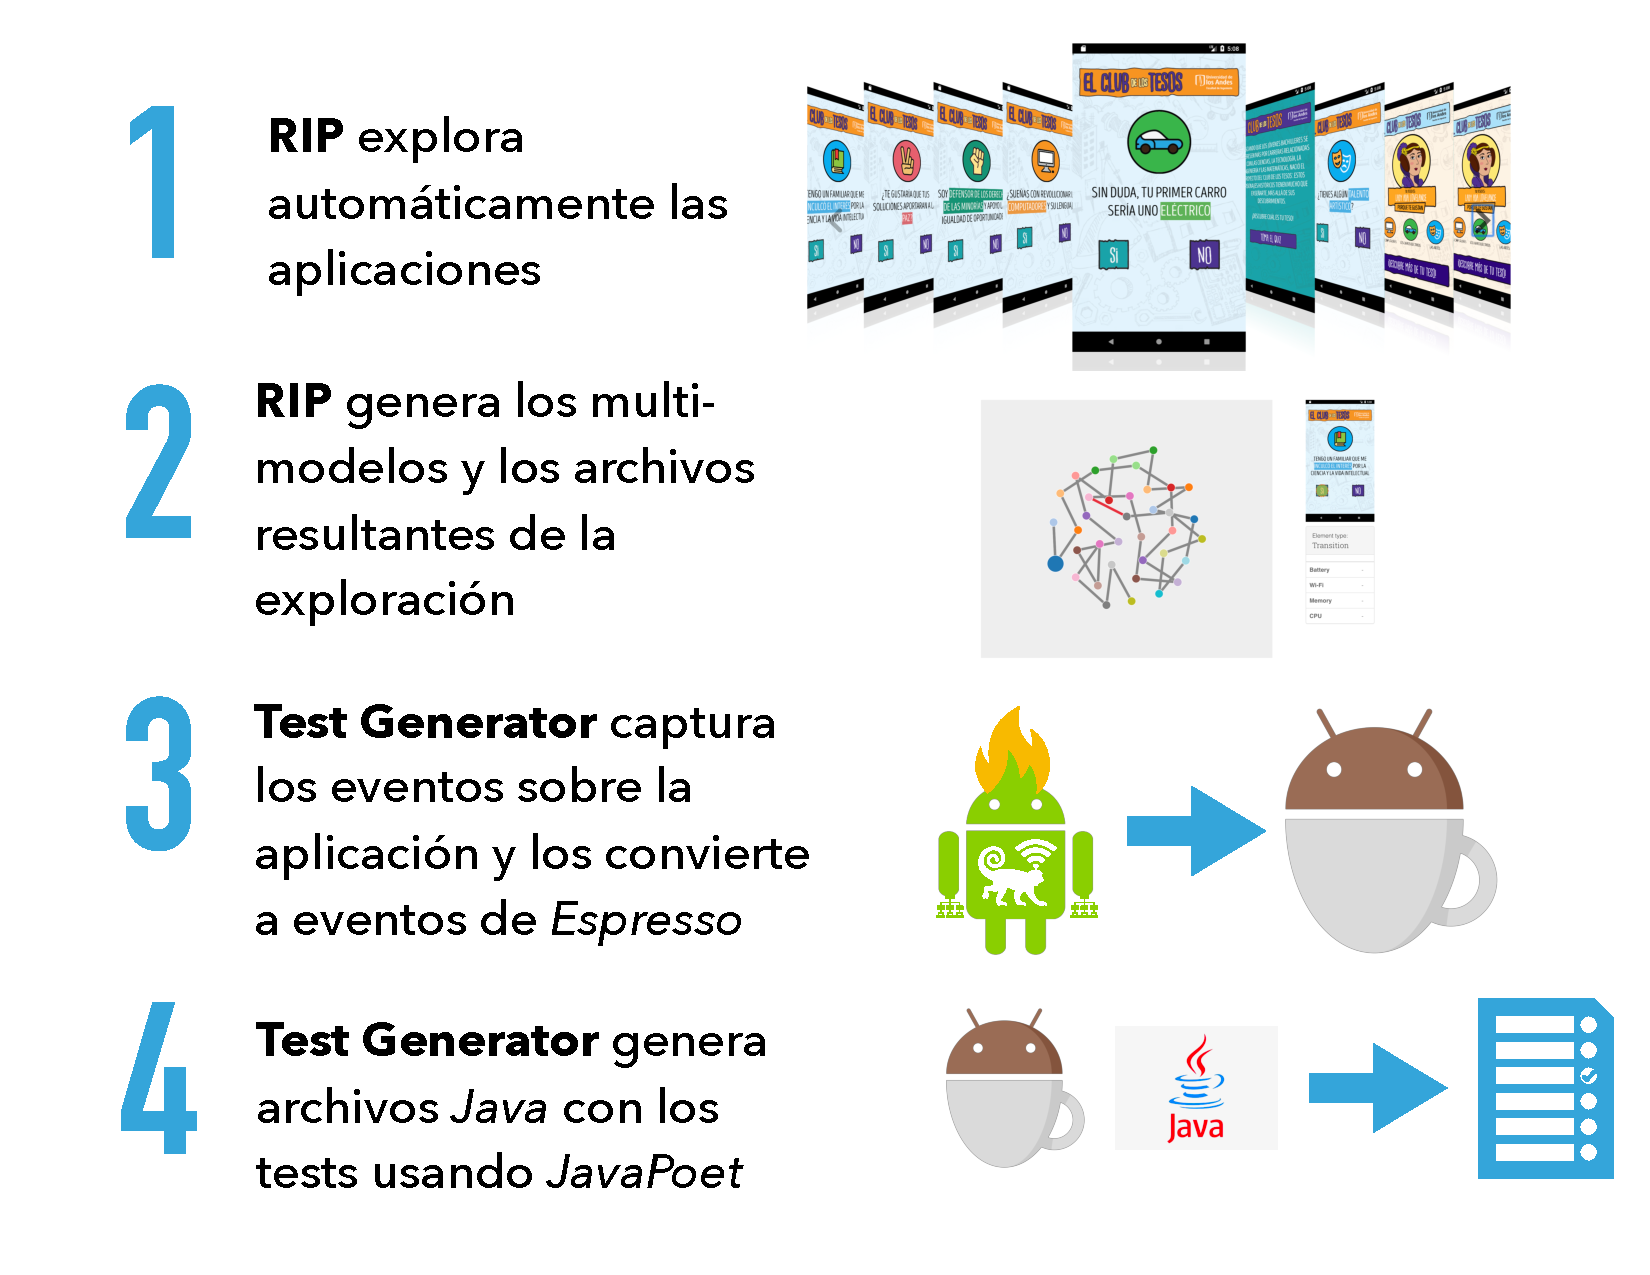
\includegraphics[width=1\textwidth]{img/procesoTests.pdf}
	\vspace{-0.5cm}
	\caption{Proceso de generación automática de tests}
	\label{procesoTests}
\end{figure} 


\section{Requisitos técnicos para la generación automática de pruebas}

\section{Generación automática de una prueba}

\section{Descripción de las pruebas generadas}
	
